% !TEX root = ../thesis.tex
% !TEX spellcheck = en-US

%% In a thesis, every section starts a new page, hence \clearpage
\clearpage

\section{Exploration and Problem Definition *}
\label{sec:Exploration}

\subsection{Project Brief}
\label{sub:Project Brief}

The objective of this thesis was to find interesting and novel ways to use the various data that get generated through Sanoma's  recruitment platform \emph{Oikotie Työpaikat}. This was stated in the research plan as follows:

\blockquote{Find an application of data mining / machine learning to the customer-generated data on the recruitment platform Oikotie Työpaikat which has the potential of bringing value to the user of the platform and is technically feasible in the scope of a master’s thesis. Further define and investigate a research problem that is essential to this application by researching literature and previous work on similar problems trying different approaches based on the literature using the results and learnings to create an improved approach.}



% - brief
% - given data
% - interest?
% - approach
% - found problem: predicting audience and popularity of job ads
% - in order to do so: learn about structure of job ads
% - problem setting as supervised task,
% - get data by free collection:
%   - to predict paragraphs
%   - to learn about how humans interpret and carry out this task
% - experiments: grouping tags automatically vs manually
% - predicting with tf.idf
% - reading up on how to write good job ads
% - can be grouped into 6 categories
% - framed as new mulit-class problem and setting up data collection
% - results: distribution and statistics, most of the data can somewhat go into these categories (other is the smallest amount)
% - then trying to evaluate the best method or combination of methods



\subsection{Approach}
\label{sub:Approach}

\subsection{Understanding structure of job ads}
\label{sub:Understanding structure of job ads}

% # personnel selection
% \cite{Chien:2008aa} - improving personnel selection with data mining
% \cite{Saidi-Mehrabad:2007aa} - The development of an expert system for effective selection and appointment of the jobs applicants in human resource management.
% \cite{Hokey-Min:2003aa} - Developing the profiles of truck drivers for their successful recruitment and retention: A data mining approach.
% \cite{Youyou:2015aa} - Computer-based personality judgments are more accurate than those made by humans
%
% # careers
% \cite{Shahaf:2012aa} - metro maps of science
%
% # formal vs informal language
% \cite{Faruqui:2011aa} - I Thou Thee, Thou Traitor": Predicting Formal vs. Informal Address in English Literature.
% \cite{Brooke:2014aa} -  Computational Approaches to Style and the Lexicon
%
% \cite{Lee:2015:RJO:2700171.2791048} - On Recommending Job Openings
%
% \cite{Luhn:1958aa} - A Business Intelligence System


\subsection{Crowdsourced Data Collection (*)}

\todo{Describe data format}

In order to perform supervised learning labelled data was needed for training. Together with the process of reframing of the research problem this was approached in an iterative way. First a quick prototypical tool was built to collect labels in a crowd-sourced fashion. This allowed getting more knowledge about the problem itself, especially with regards to how humans perform the task of labelling topics of text sections, and to perform first experiments of algorithmically achieving meaningful results in agreement to human behavior on this task.
Then these learnings were taken into consideration when re-scoping the research problem and according to that data was collected using the micro tasking service CrowdFlower\footnote{\textquote{CrowdFlower is a data enrichment, data mining and crowdsourcing company [\ldots]. The company's software as a service platform allows users to access an online workforce of millions of people to clean, label and enrich data.} Source: \url{https://en.wikipedia.org/wiki/CrowdFlower}, Company website: \url{https://www.crowdflower.com}}, leading to a quality dataset of labelled sentences from job ads.

\subsubsection{Explorative Paragraph Dataset}

\todo{Picture of software setup?}

To collect first data a tool was build, consisting of a Node.js\footnote{[\ldots] Node.js is an open-source, cross-platform runtime environment for developing server-side Web applications. \url{https://nodejs.org/}} server using MongoDB\footnote{\textquote{MongoDB is a free and open-source cross-platform document-oriented database [\ldots].} Source: \url{https://en.wikipedia.org/wiki/Node.js}, Website: \url{https://www.mongodb.com}} as a database and communicating via a JSON with a simple website front-end using the mustache template engine\footnote{\textquote{Mustache is a simple web template system.} Source: \url{https://en.wikipedia.org/wiki/Mustache_(template_system)}, Website: \url{https://mustache.github.io}}.
The tool is online\footnote{\url{http://thesis.cwestrup.de/jobad-tagger/}} and it's source code is publicly available on GitHub\footnote{\url{https://github.com/cle-ment/thesis-tagger}} with it's API documentation hosted online as well\footnote{\url{http://thesis.cwestrup.de/jobad-tagger/apidoc/}}.

The data generated by using the free-form text description of each job ad and splitting it into paragraphs as can be seen in the software package as well\footnote{\url{https://github.com/cle-ment/thesis-tagger/blob/master/pre-processing.ipynb}}.

The goal of this prototype tool for data collection was on the one hand to acquire data in order to carry our first experiments as fast as possible, and on the other hand to gain a deeper understanding about the research problem itself by giving an open, unbiased task to the participants. In particular the question at hand was how humans label the content of the different parts of a job ad.

The exact task given to the participants was ``Describe what each section is about by adding one or more tags/keywords to it''. They were shown a job ad that was split into paragraphs and besides each paragraph was a text field to enter 1 or more tags.

\begin{figure}[h]
  \centering
  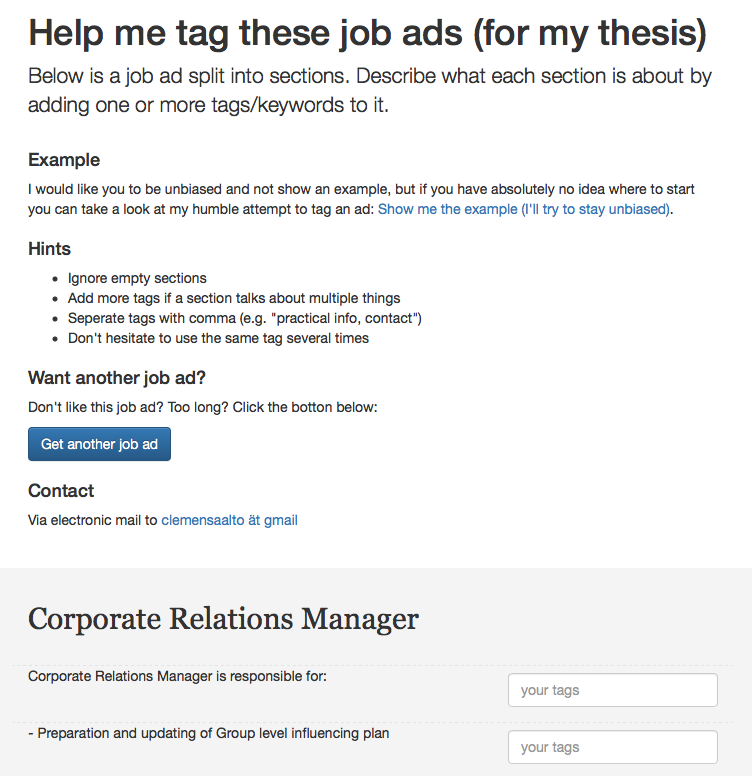
\includegraphics[width=\textwidth]{img/thesis-tagger-interface.png}
  \caption{Screen capture of the interface of the tagging tool}
\label{fig:thesis-tagger-interface}
\end{figure}

In a first step the tool was only shown to 3 participants to get immediate feedback if the user interface had flaws and whether the task was understood.   Based on this feedback the tool was improved by providing an example for the participants and then tested with a slightly larger group of 12 persons. After correcting a few minor details in the user interface a public link was then shared via social media and other channels with as many people as possible. A few days later the tool was then also shared internally within Sanoma where it was set up as a competition to tag the most possible job ads.

In total 91 job ads were tagged, resulting in 379 tagged text sections and 358 tags.

\todo{Describe data: Different characteristics}
\todo{show distribution?}
\todo{show embedding visualizations}

\begin{figure}[h]
    \centering
    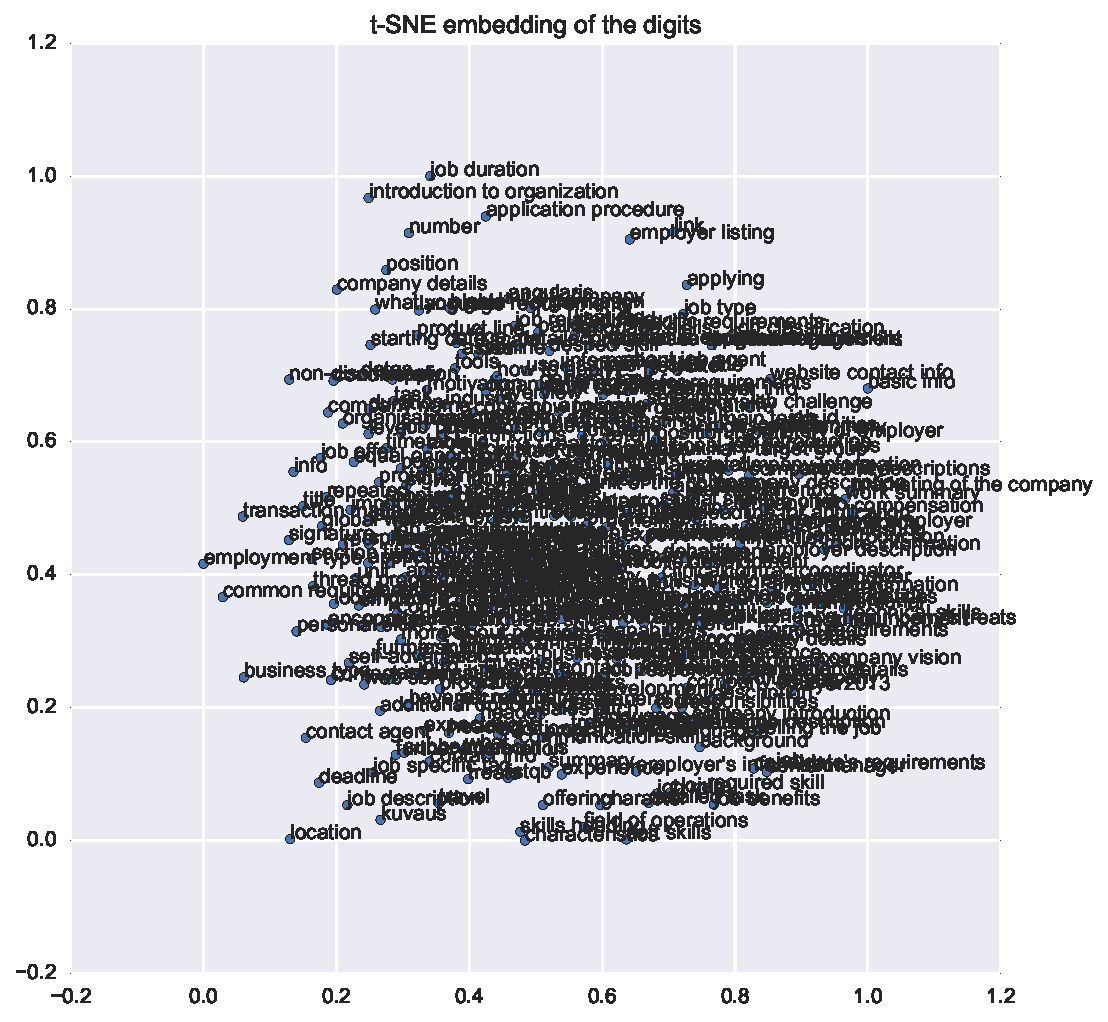
\includegraphics[width=\textwidth]{img/paragraph-data-tSNE.pdf}
    \caption{t-SNE Embedding}
\label{fig:paragraph-data-tSNE}
\end{figure}

\begin{figure}[h]
    \centering
    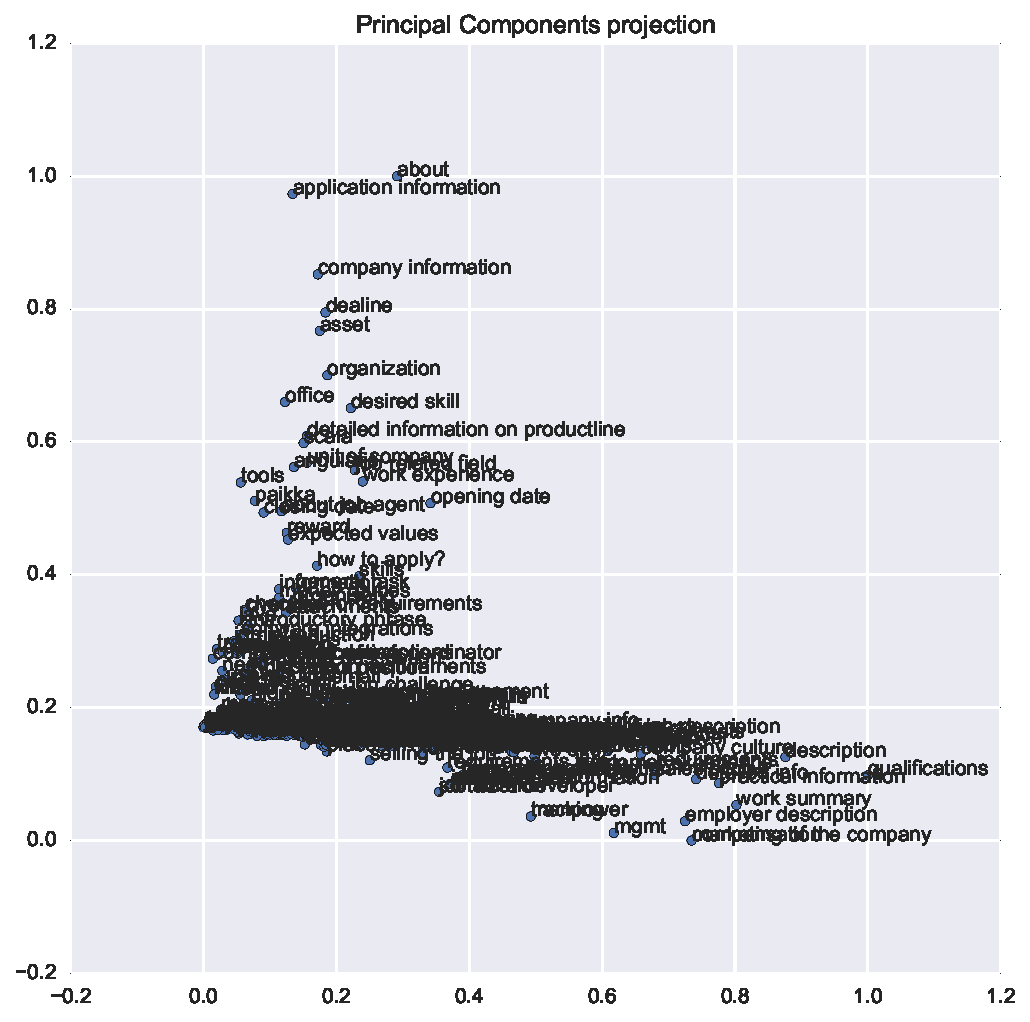
\includegraphics[width=\textwidth]{img/paragraph-data-principal-components-projection.pdf}
    \caption{Principal Components Projection}
\label{fig:paragraph-data-principal-components-projection}
\end{figure}

\todo{Comparison one-vs-rest and one-vs-one against linear machine}
\todo{Visualizations and embeddings of data in 2D (and decision boundaries?)}
\todo{show T-SNE embeddings of doc2vec vectors}
